% Chapter 2

\chapter{Background Theory} % Main chapter title

\label{Chapter2} % For referencing the chapter elsewhere, use \ref{Chapter1} 

\lhead{Chapter 2. \emph{Background Theory}} % This is for the header on each page - perhaps a shortened title

%------------------------

--------------------------------------------------------------------------

Autonomous vehicular systems are adopting lane detection as a part of their driving assistance systems. Lane detection is to detect lanes on the road and provide the accurate location and shape of each lane. It serves as one of the key techniques to enable modern assisted and autonomous driving systems. One of the principal approaches to lane detection is the accurate detection of road boundaries and lanes using a vision system however it is a difficult problem due to varying road conditions. To train the vision systems for different sets of vehicular systems (aircrafts, motor cycles, cars), huge amounts of dataset are required for the individual systems. We propose a unified machine learning model enhanced by transfer learning which would assist artificial intelligent systems in autonomous driving systems.


\section{Artificial Intelligence}


Artificial intelligence (AI) refers to machines' creative ability to assess data and make intelligent decisions, implying that they can make decisions and perform tasks based on data in the same way that humans do. The world is changing at a rapid pace, with Artificial Intelligence at the forefront of transforming the environment and how we live. AI and self-driving cars are becoming more common in our daily lives and primary industries. It is an area of computer science concerned with intelligent machine behavior and a machine's cleverly simulated ability to mimic human actions and reaction patterns. Artificial intelligence is being more widely used in the field of driving, which is beneficial to driverless vehicles and the Advanced Driver Assistance System (ADAS). For instance, ADAS have been categorized into different levels based on the amount of automation, and the scale provided by The Society of Automotive Engineers (SAE).\cite{8633345} There are five distinguished levels of ADAS. At Level 0, ADAS cannot control the vehicle and can only supply information for the driver to understand on their own. The various examples of Level 0 can be given as parking sensors, surround-view, traffic sign recognition, lane departure warning, night vision, blind spot information system, rear-cross traffic alert, and forward-collision warning. The following Level 1 and 2 are very identical to each other where the driver has the control to make majority of the decision. The only The distinction between the two levels is that Level 1 can manage one capability while Level 2 can control numerous to assist the driver.\cite{8633345}. Some examples of Level 1 ADAS include adaptive cruise control, emergency brake aid, automated emergency brake help, lane maintaining, and lane centering where as Level 2 ADAS include highway aid, autonomous obstacle avoidance, and automated parking. Level 3 to 5 ascends with the increased control of the degree of supervision in accordance to the vehicle with Level 5 being entirely autonomous. Lane detection, as a fundamental challenge in autonomous driving, is crucial in applications including vehicle real-time positioning, driving route planning, lane keeping aid, and adaptive cruise control. 

In terms of both the diversity of potential applications and the levels of interest among conventional actors in the automotive, truck, public transportation, industrial, and military communities, the field of intelligent vehicles is quickly expanding around the world. Intelligent vehicle (IV) solutions have the potential to improve safety and operating efficiency significantly. As a component of intelligent transportation systems (ITS), IV systems use a distinct sensor in conjunction with an intelligent algorithm to analyze the surrounding environment in order to either aid the driver in vehicle operations (driver assistance) or totally operate the vehicle.\cite{1364006}

Modern automobiles include an increasing variety of driver assistance capabilities, like automatic lane maintaining. The latter enables the vehicle to correctly position itself within the road lanes, which is also critical for any later lane departure or trajectory planning choice in fully autonomous vehicles. Traditional lane detection systems rely on a combination of highly specialized, hand-crafted features and heuristics, which are frequently followed by post-processing procedures that are computationally expensive and susceptible to scalability due to road scene fluctuations. Fully autonomous vehicles are currently the primary focus of computer vision and robotics research, both at the academic and industrial levels. The goal in each scenario is to gain a complete understanding of the world around the car by utilizing numerous sensors and control modules. Camera-based lane recognition is a crucial step toward such environmental perception since it allows the car to place itself correctly inside the road lanes. It's also important for each subsequent lane departure or trajectory planning decision. As a result, reliable camera-based lane recognition in real-time is a critical enabler of fully autonomous driving.\cite{neven_towards_2018}

AI is an important factor in this entire equation as it is the decision maker which has been trained based on various selected machine learning algorithms and this process has been enhanced with transfer learning to bring in higher efficiency and precision. 
%----------------------------------------------------------------------------------------

\section{Machine Learning}


Machine learning is a branch of artificial intelligence and computer science that focuses on using data and algorithms to replicate how humans learn, gradually improving its accuracy. Artificial intelligence systems are used to solve complex problems in a way that is similar to how humans solve problems. If an agent improves its decision making with each iteration by retaining information or making observations in the current environment, it is said to be learning. It is the process through which an agent adapts to new situations, discovers, and extrapolates patterns in the given universe. 


The swift and steady development and adoption of high-precision optic and electronic sensors has called for high-efficiency and high-effective computer vision and machine learning algorithms which provide real-time driving scene analysis. Current research has been based on developing advanced algorithms for driving scene interpretation, with the goal of developing either an autonomous car or an advanced driver aid system (ADAS). Prior to the development of self-driving cars, automobiles had Active Lane Tracking Assistance. Because of the scarcity of self-driving cars, several well-known automobile manufacturers adopt this method. This system may be used in a variety of ways. These are just sound and vibration warnings, steering interventions in place of the driver, and so on. This technology aids in keeping the car in its lane. As a result, the significance of lane tracking system is realized.\cite{kamci_lane_2019} Lane detection is one of the most fundamental study areas which has been focused on as part of the autonomous driving aided systems. To develop an artificial intelligent interface, we need machine learning to make it accurate with the highest efficiency and precision. \cite{zou_robust_2020} 




\section{Transfer Learning}

Transfer learning is a useful approach in machine learning for dealing with the fundamental problem of  insufficient training data. It attempts to transfer knowledge from the source domain to the target domain by reducing the requirement that the training and test data be i.i.d. This will have a significant beneficial impact on many areas that are difficult to develop due to a lack of training data. Figure 1 depicts the transfer learning learning process. Some of the terms used in this survey should be defined.


\begin{figure}[htbp]
	\centering
		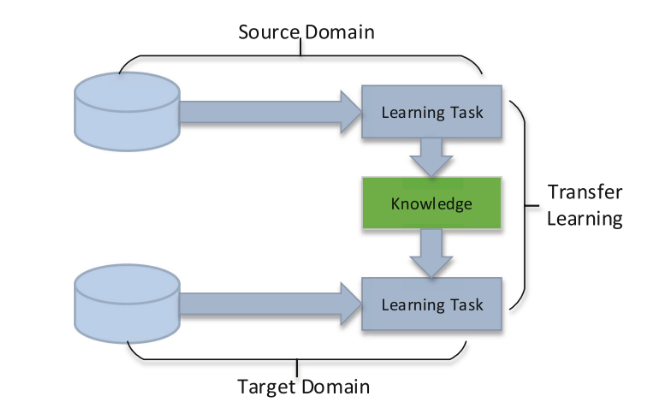
\includegraphics[scale=0.5]{Figures/process1.png}
		\rule{35em}{0.5pt}
	\caption[The Transfer Learning Process]{Learning process of transfer learning.}
	\label{fig:Transfer Learning Process}
\end{figure}


First of all, we give the definitions of a domain and a task respectively: A domain can be represented by D = {$\chi$, P(X)}, which contains two parts: the feature space $\chi$ and the edge probability distribution P(X) where X = {$x_1$, ..., $x_n$} $\in$ $\chi$. A task can be represented by T = {y, \emph{f(x)}}. It consists of two parts: label space \emph{y} and target prediction function \emph{f(x)}. \emph{f(x)} can also be regarded as a conditional probability function {P(y $\mid$ x)}. Then, the transfer learning can be formal defined as follows:

\emph{Definition 1 (Transfer Learning): Given a learning task $T_t$ based on $D_t$ and we can get the help from $D_s$ for the learning task $T_s$. Transfer learning aims to improve the performance of predictive function $f_T$ (·) for learning task $T_t$ by discover and transfer latent knowledge from $D_s$ and $T_s$, where $D_s$ = $D_t$ and/or $T_s$ = $T_t$. In addition, in the most case, the size of $D_s$ is much larger than the size of $D_t$, $N_s$, $N_t$.}\cite{tan2018survey}

Transfer learning offers the capacity to transfer information from a simulated domain to a real-world setting. Transfer learning works well when data from various feature spaces or domains is used to train a model. Machine learning applications frequently need a significant amount of real-world data. Inadequate data may be compensated for by producing simulated data in the virtual world and applying transfer learning to bridge the gap.\cite{akhauri2020enhanced} By transferring information from a similar subject, transfer learning can boost learning. For example, knowledge in mathematics and statistics can aid in understanding of machine learning ideas. Transfer learning research has focused on adapting to new domains, applications, and methodologies throughout the previous decade. "A Survey of Transfer Learning" by Karl Weiss\cite{5288526} explicitly defines transfer learning, discusses the current state of the art, and examines transfer learning applications. In particular, we investigate the application of transfer learning in autonomous driving, with an emphasis on transfer from the different world domains.

A large amount of training data is required for a model to achieve appropriate accuracy. A large amount of training data is required for a model to achieve appropriate accuracy. Transfer Learning is one solution to this problem. Transfer learning occurs when a network or model is trained on one dataset and one task and then utilized to train on another dataset and task. When a network is trained on pictures, the earliest layers tend to learn low-level characteristics such as edges, lines, and corners. Because it occurs regardless of whatever dataset is utilized, these characteristics are referred to as universal features.
We apply the fine-tuning technique, which replaces not only the classifier but also the weights in the previous layers for weight initialization. The network is then retrained with the fresh dataset and a new classifier is added on top. It is called fine-tuning because the weights are modified from the place they were in the pre-trained network to match the new dataset rather than being trained from start. It is also possible to freeze the previous layers, which means they are no longer trainable; however, because the earlier layers consist of generic characteristics, they may be left alone. Only the more specific properties of the previous dataset are changed in this scenario to better match the new job and dataset.\cite{strömgren}

Researchers utilize transfer learning for object detection due to the scarcity of labelled data and the time necessary to label the data. Lim et al. \cite{lim_1970} used transfer learning to develop a unique strategy for accommodating limited training data examples in a certain class.This is where transfer learning will contribute to universalising the learning architecture. Using autonomous cars as the base case, we can use transfer learning to generate models for other vehicular systems. During the early stages of literature review, we can assert that transfer learning can be used in the proposed system and modularized during the lane detection phase for a particular system as well as transferring model knowledge to other vehicular systems. 